\chapter{Revisão de literatura}\label{chap:revisao}

Nesta seção deve-se inserir os achados da revisão de literatura. Caso o trabalho contenha uma fundamentação teórica, pode-se inserir ela como uma sub-seção aqui. Mesmo que não seja realizado um processo sistemático é interessante que o processo de busca e de triagem sejam claros e descritos de forma que possam ser reproduzidos.  Acrescente aqui ainda questões relativas à descrição do sistema/uso atual, enfatizando as partes que vai abordar no seu trabalho.

\section{Fundamentação Teórica}

Descreva nesta seção os conhecimentos, fora da área de Tecnologia da Informação, que são necessários ao entendimento do seu trabalho. Lembre-se de mencionar as fontes consultadas para a aquisição do conhecimento e escrita da fundamentação.


\section{Dicas para Citações e Referências Bibliográficas}


As citações são indicativos a quem vai ler seu texto de onde você buscou aquele conhecimento/conteúdo, com vistas a escrita de seu texto. Em geral, as citações podem ser de duas formas: diretas ou indiretas. Elas remetem às referências bibliográficas.

As referências bibliográficas neste modelo (em \LaTeX) são automaticamente inseridas com o uso dos comandos ``\texttt{\textbackslash cite}'' e suas variações. O correto preenchimento da sua base de referências, em formato ``\texttt{\textbackslash cite}'' mantém seu texto com as referências corretamente formatadas.

\subsection{Citações diretas}

Para uma \textbf{citação direta} use o comando ``\texttt{\textbackslash cite}''. A citação deve iniciar e terminar por aspas duplas. Se o texto original já contiver aspas duplas, substituí-las por aspas simples (apóstrofos). Em citações diretas, pode-se adicionar o número da página ou localização, se houver, após o ano (neste caso, use o comando ``\texttt{\textbackslash citet}''). Os próximos itens apresentam alguns exemplos:

\begin{itemize}
    \item Segundo \citet[p.~27]{RIE11}, ``medidas fisiológicas ainda não podem ser consideradas como substitutas de medidas de desempenho e de avaliação subjetiva'';
	
    \item De acordo com \cite{Lopes2023} ``foi definido que...'';

    \begin{itemize}
        \item \cite{patricio2018computer} afirmam que ``a produção de grãos desempenha um papel importante na economia global'';
        
        \item ``A OpenGL é uma API complexa, com muitos detalhes que podem confundir o iniciante'', conforme mencionado por \citet[cap.~3]{COH06}.
    \end{itemize}
\end{itemize}

Para uma \textbf{citação direta com mais de três linhas} ela deve ser destacada com recuo de 4 cm da margem esquerda, com letra menor que do que a utilizada no texto. Não se utilizam aspas. A indicação da página da citação pode estar inserida ao final do texto citado. Veja o exemplo a seguir:

Sobre o caderno de campo para dispositivos móveis, \cite{SIL13} consideram que:
% Comando para citação direta. Mantenha sem endentação no início da frase, para que não seja aplicado o espaçamento de primeira linha.
\begin{directcite}
	\noindent Para preencher a lacuna entre aplicações nativas e web, mantendo a portabilidade da solução, faz-se necessário o uso de uma abordagem de desenvolvimento híbrido, em que tecnologias web (HTML, CSS, Javascript) são utilizadas em conjunto com recursos nativos de uma interface de programação (p. 2).
\end{directcite}

É conveniente que após uma citação direta, o autor do texto que está realizando a citação, utilize da informação citada para realizar ligação ou complementar a idea de seu texto. Uma citação direta solitária e isolada, não faz muito sentido no seu texto.

\subsection{Citações indiretas}

Para uma \textbf{citação indireta} use o comando ``\texttt{\textbackslash citep}''. Não se utilizam aspas para esse tipo de citação, nem a(s) página(s) de onde foi extraída a ideia. Este é um dos formatos mais utilizados em monografias, pois apresenta a ideia de outros autores utilizando suas próprias palavras:

\begin{enumerate}[label=\alph*)]
	\item A biblioteca jDssat permite a integração com o DSSAT com novas interfaces \citep{Resenes2019};
	\item Redes de Petri podem ser utilizadas para especificar uma tarefa de interação, possibilitando identificar partes de código reutilizáveis em novos projetos de interfaces de Realidade Virtual~\citep{RIE10}.
\end{enumerate}

Já na \textbf{citação de citação} a indicação da fonte é iniciada pelo sobrenome do autor da obra citada (não consultada). Em seguida, dentro de parênteses, utiliza-se a expressão latina \textit{apud} ou citado por, seguido do sobrenome do autor da obra consultada. Quando for citação direta, utilizar aspas. Tome por base o exemplo a seguir:
\begin{itemize}
	\item Segundo \cite{BOW02} (\textit{apud}~\cite{BOW04}), as técnicas para manipulação 3D podem ser classificadas de maneira isomórfica, por decomposição de tarefas e por metáfora de interação.
\end{itemize}

Para a \textbf{Indicação de Citação} são apresentados os seguintes exemplos:

\begin{itemize}
	\item \textbf{Exemplo com autor pessoal}
	\\ De acordo com \cite{COM10}, apesar da precaução tomada em relação à preparação da pele, aplicação do gel condutor, colocação dos eletrodos e instruções ao usuário, é muito difícil gravar dados de frequência cardíaca absolutamente livre de ruídos;

	\item \textbf{Exemplo com dois autores}
	\\ \cite{COH06} destacam que a OpenGL é uma biblioteca de rotinas gráficas e de modelagem 2D e 3D, portável, rápida e que permite desenvolver aplicações interativas com alto grau de realismo;
	
	\item \textbf{Exemplo com três ou mais autores} 
	\\ Neste contexto, \cite{BOW04} afirmam que a Realidade Aumentada é uma área em expansão para novas e desafiadoras soluções;

	\item \textbf{Exemplo com referência à duas ou mais obras}
	\\ Lorem ipsum é um texto fictício, composto por palavras em latim que, embora não tenham um significado coerente, simula a estrutura e o fluxo de um texto real \citep{RIE111, BENTLEYBC07};
	
	\item \textbf{Exemplo com autor institucional}
	\\ De acordo com o site da UPF \citep{UPF24}: ``Há 55 anos, a Universidade de nossa comunidade'';
	
	\item \textbf{Exemplo sem autor, com a entrada pelo título} \\Segundo o manual de Referência do GTK+~3~\citep{GTK13}, a última versão estável é a 3.10.6.
\end{itemize}

Para a exibição correta do \textbf{Digital Object Identifier (DOI)}, quando a referência possuir, use no bibitem da referência o campo ``\texttt{note}'' da seguinte forma ``\texttt{note=\{\textbackslash url\{url completa do DOI\}\}}''. Não use os campos ``\texttt{doi}'' ou ``\texttt{url}''.

Quando do uso da \textbf{URL}, quando se quiser indicar a disponibilidade de uma referência, use no bibitem da referência o campo ``\texttt{note}'' da seguinte forma ``\texttt{note=\{Disponível em \textbackslash url\{url\_completa\_da\_referência\}\}}''. Não use o campo ``\texttt{url}''.

Para casos em que o primeiro autor seja o mesmo para dois ou mais trabalhos, publicados no mesmo ano, é necessário adicionar identificadores no campo ``\texttt{year}'', no bibitem de cada referência relacionada. Por exemplo, ``\texttt{year=\{2020a\}}'' na entrada referente ao primeiro trabalho deste primeiro autor publicado em 2020, ``\texttt{year=\{2020b\}}'' para o segundo trabalho dele em 2020, e assim por diante.
\\
\section{Tabelas, Quadros, Algoritmos, Figuras, Equações, Seções e Capítulos}

Para que os elementos desta seção possam ser citados, eles necessitam ser identificados quando inseridos no texto. Para tanto, deve-se utilizar a \textit{tag} ``\texttt{\textbackslash label[nome]}'', substituindo o \texttt{nome} pela identificação do elemento. Este \texttt{nome} deve ser único no documento e em geral se inicia pelo tipo (\texttt{tab} para tabelas, \texttt{fig} para figuras ...), seguido de ``:'' e um identificador.

Seguem exemplos:
\begin{enumerate}[label=(\Roman*)]
	\item \textbf{Citação}: para referenciar os itens acima no texto use ``\texttt{\textbackslash cref}''. As palavras (Figura, Tabela, Equação, Seção, Capítulo) das citações aparecem automaticamente antes do seu respectivo número, não é necessário escrevê-las;
	
	\item \textbf{Tabelas e Quadros}: adota-se uma simplificação relativa à Norma ABNT, não fazendo diferença entre tabelas e quadros. Ambos os casos devem ser considerados tabelas. A legenda deve ser centralizada, não usar negrito, e deve estar posicionada sobre a tabela. Exemplos podem ser visualizados na \cref{tab:tab1} e na \cref{tab:tab2} (ou nas \cref{tab:tab1,tab:tab2} ou nas \crefrange{tab:tab1}{tab:tab2});
	
	% Você pode montar suas tabelas on-line e gerar o código. Alguns links para ajudar:
	% http://www.tablesgenerator.com/
	% http://truben.no/latex/table/
	
	\begin{table}[H]
		\centering
		\caption[Preços de alimentos em dólares de 1950-1952 a 1995-1997.]{Preços de alimentos em dólares de 1950-1952 a 1995-1997~\citep{DET70}.}
		\label{tab:tab1}
		\begin{tabular}{lrrc} \hline
			\textbf{Alimento} & \textbf{1950-1952} & \textbf{1995-1977} & \textbf{Variação} \\ \hline
			Trigo    & 427,6     & 159,3     & -62,7\%  \\
			Arroz    & 789,7     & 282,3     & -64,2\%  \\
			Sorgo    & 328,7     & 110,9     & -66,2\%  \\
			Milho    & 372,0     & 119,1     & -68,0\%  \\ \hline
		\end{tabular}
	\end{table}
	
    \begin{table}[H]
      \centering
      \footnotesize
      \caption[Quadro comparativo de competitividade.]{Quadro comparativo de competitividade~\citep{MAL00}.}
      \label{tab:tab2}
      \begin{tabular}{|l|l|l|l|}
      \hline
      \rowcolor[HTML]{C0C0C0} 
      \textbf{Empresa} & \textbf{\begin{tabular}[c]{@{}l@{}}Principal\\ Matéria-Prima\end{tabular}} & \textbf{\begin{tabular}[c]{@{}l@{}}Alternativas de Suprimentos\\ para a Principal Matéria-Prima\end{tabular}} & \textbf{Flexibilidade} \\ \hline
      Copesul          & Nafta                                                                      & Disponibilidade de produto na Argentina                                                                       & 45\% condensado e GLP  \\ \hline
      Copesul          & Nafta                                                                      & Alternativas Venezuela e Argélia                                                                              & Inexistente            \\ \hline
      PQU              & Nafta                                                                      & Único fornecedor                                                                                              & Inexistente            \\ \hline
      Rio Polímeros    & Etano                                                                      & Único fornecedor                                                                                              & Inexistente            \\ \hline
      Baía Blanca      & Etano                                                                      & Projeto Mega / Única Opção                                                                                    & Inexistente            \\ \hline
      Baía Roja        & OMG                                                                        & Oh Long Johnson                                                                                               & 100\%                  \\ \hline
      \end{tabular}
    \end{table}
	
	\item \textbf{Figuras}: adota-se uma simplificação relativa à Norma ABNT, não fazendo diferença entre figuras e gráficos. Ambos os casos devem ser considerados figuras. Pseudocódigos ou trechos de código-fonte também devem ser referenciados como figuras. A legenda deve ser centralizada, não usar negrito, e deve estar posicionada sob a figura. Exemplos podem ser visualizados na \cref{fig:fig1}, na \cref{fig:fig2} e na \cref{fig:codigoc} (ou nas \cref{fig:fig1,fig:fig2,fig:codigoc}). Para ignorar citações nas legendas nas listas de figuras e de tabelas, deve-se adicionar uma legenda reduzida como primeiro argumento no comando \textit{caption} sem a citação. Um exemplo pode ser visto na descrição da \cref{fig:fig1}. Agora, um exemplo de figura de dimensões grandes ou maior resolução, ajustada para ser exibida exatamente a largura entre margens, como mostra a \cref{fig:conceito4}. E, por fim, a \cref{fig:lis} mostra um exemplo de inserção de subfiguras, apresentados pela \cref{fig:lis}\subref{fig:lis1} e pela \cref{fig:lis}\subref{fig:lis2};
	
	\begin{figure}[htb!]
		\centering
		
\includegraphics[width=\textwidth]{fig/PPGCA_logo_UPF_10anos_web-01}
		\caption[Banner de divulgação dos 10 anos do PPGCA.]
		{\label{fig:conceito4}Banner de divulgação dos 10 anos do PPGCA.}%
	\end{figure}

        \todo[inline]{Este comando é útil para deixar comentários bem visíveis no texto}

        % OBS.: ao invés de usar figuras matriciais de alta resolução (JPG, PNG), ou figuras vetoriais em formato EPS, você pode incluir versões das figuras no formato PDF. Mantém a alta qualidade, e favorece um melhor desempenho durante a compilação do documento.
	\begin{figure}[!htb]
		\begin{center}
			\subfigure[Flor de lis azul.]{
				\label{fig:lis1}
				
\includegraphics[width=.25\textwidth]{fig/royal-blue-fleur-de-lis.eps}
			}
			\subfigure[Flor de lis vermelha.]{
				\label{fig:lis2}
				
\includegraphics[width=.25\textwidth]{fig/blood-red-fleur-de-lis.eps}
			}
		\end{center}
		\caption{Duas flores de lis.}
		\label{fig:lis}
	\end{figure}
	
	\todo[inline]{É possível criar uma relação desses comentários. Há um exemplo logo após o sumário.}
    
	% Um exemplo de figura
	\begin{figure}[htb!]
		\centering
\includegraphics[scale=0.25]{fig/logo-color-horizontal-complemento.png}
		\caption[Logotipo da Universidade (adaptado do site da UPF).]
		{\label{fig:fig1}Logotipo da Universidade (adaptado do site da UPF)~\citep{UPF24}.}%
	\end{figure}

    
	% Um exemplo de figura
	\begin{figure}[htb!]
		\centering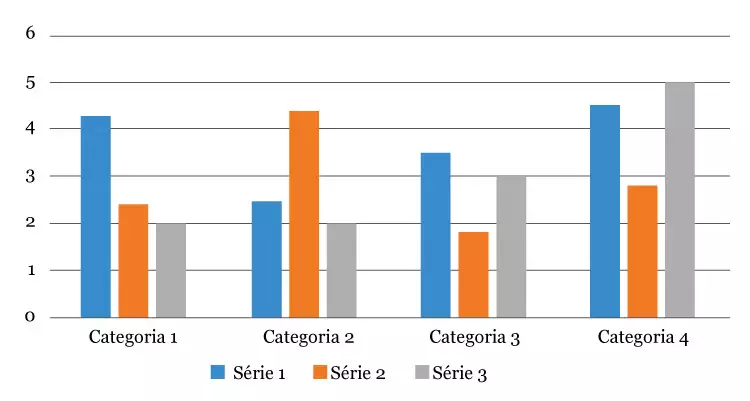
\includegraphics[width=9.18cm,height=4.91cm]{fig/graficoBonitinho.jpg}
		\caption%[This figure has a shorter caption now]%
		{\label{fig:fig2}Uma imagem qualquer de um gráfico de barras.}%
	\end{figure}
    
    \todo[inline]{Nas estruturas como figuras, tabelas, algoritmos, listas ou equações é interessante que elas sejam citadas e após comentadas}
    	
	\begin{figure}[htb!]
		\centering
		\begin{tabular}{rl} \hline
			\texttt{1.} & \texttt{\#include <iostream>}  \\
			\texttt{2.} & \texttt{using namespace std;}  \\
			\texttt{3.} & \texttt{int main()}  \\
			\texttt{4.} & \texttt{\{}  \\
			\texttt{5.} & \texttt{\hspace{2ex}cout  {<}{<} "Hello World!"~{<}{<} endl;}  \\
			\texttt{6.} & \texttt{\hspace{2ex}return 0;}  \\
			\texttt{7.} & \texttt{\}}  \\ \hline
		\end{tabular}
		\caption%[This figure has a shorter caption now]%
		{\label{fig:codigoc}Código-fonte C++.}%
            %\vspace{19.6cm} % espaço vertical inserido para evitar que a figura fique posicionada no centro de uma página separada, e não no topo.        
	\end{figure}

    Um exemplo de comentário sobre a \cref{fig:codigoc} é que o código fonte apresentado representa um ... \todo{add que ....}

    \todo[inline]{O exemplo acima é outro de uso do todo. Usar ele com cuidado}
    
	\item \textbf{Equações e fórmulas}: equações e fórmulas devem ser colocadas em uma nova linha, centralizadas e numeradas consecutivamente para fins de referência, como pode ser observado na \cref{eq:baskara}.
	
	% Você pode montar suas equações on-line e gerar o código. Alguns links para ajudar:
	% https://latexeditor.lagrida.com
	% https://latex.codecogs.com/eqneditor/editor.php
	
	\begin{equation}\label{eq:baskara}
		x= \frac{-b\pm\sqrt{b^2-4ac}}{2a}
	\end{equation}
\end{enumerate}

    Outro exemplo de comentário é que a \cref{eq:baskara} representa a Equação de Baskara. O valor que deve ser calculada a raiz quadrada também é conhecido com delta.
    
    \todo[inline]{Os exemplos de comentários colocados são bem triviais. Use ele com maior qualidade dos comentários inseridos}

Dados estatísticos ou numéricos também podem ser adicionados no texto, usando um bloco com o símbolo \$ ($12,5 \pm 1,8$). Outros exemplos de referências cruzadas podem ser realizados. Exemplos: \cref{chap:revisao}.